\documentclass{article}

\usepackage{graphicx}
\usepackage{tikz}
\usepackage{tikzsymbols}
\usetikzlibrary{calc,patterns,shapes.geometric}
\pagestyle{empty}
\usepackage[margin=0pt]{geometry}
\geometry{papersize={14in,12in}}

\def\centerarc[#1](#2)(#3:#4:#5){\draw[#1] ($(#2)+({#5*cos(#3)},{#5*sin(#3)})$) arc (#3:#4:#5);}

\begin{document}
	\begin{figure}
		\centering
		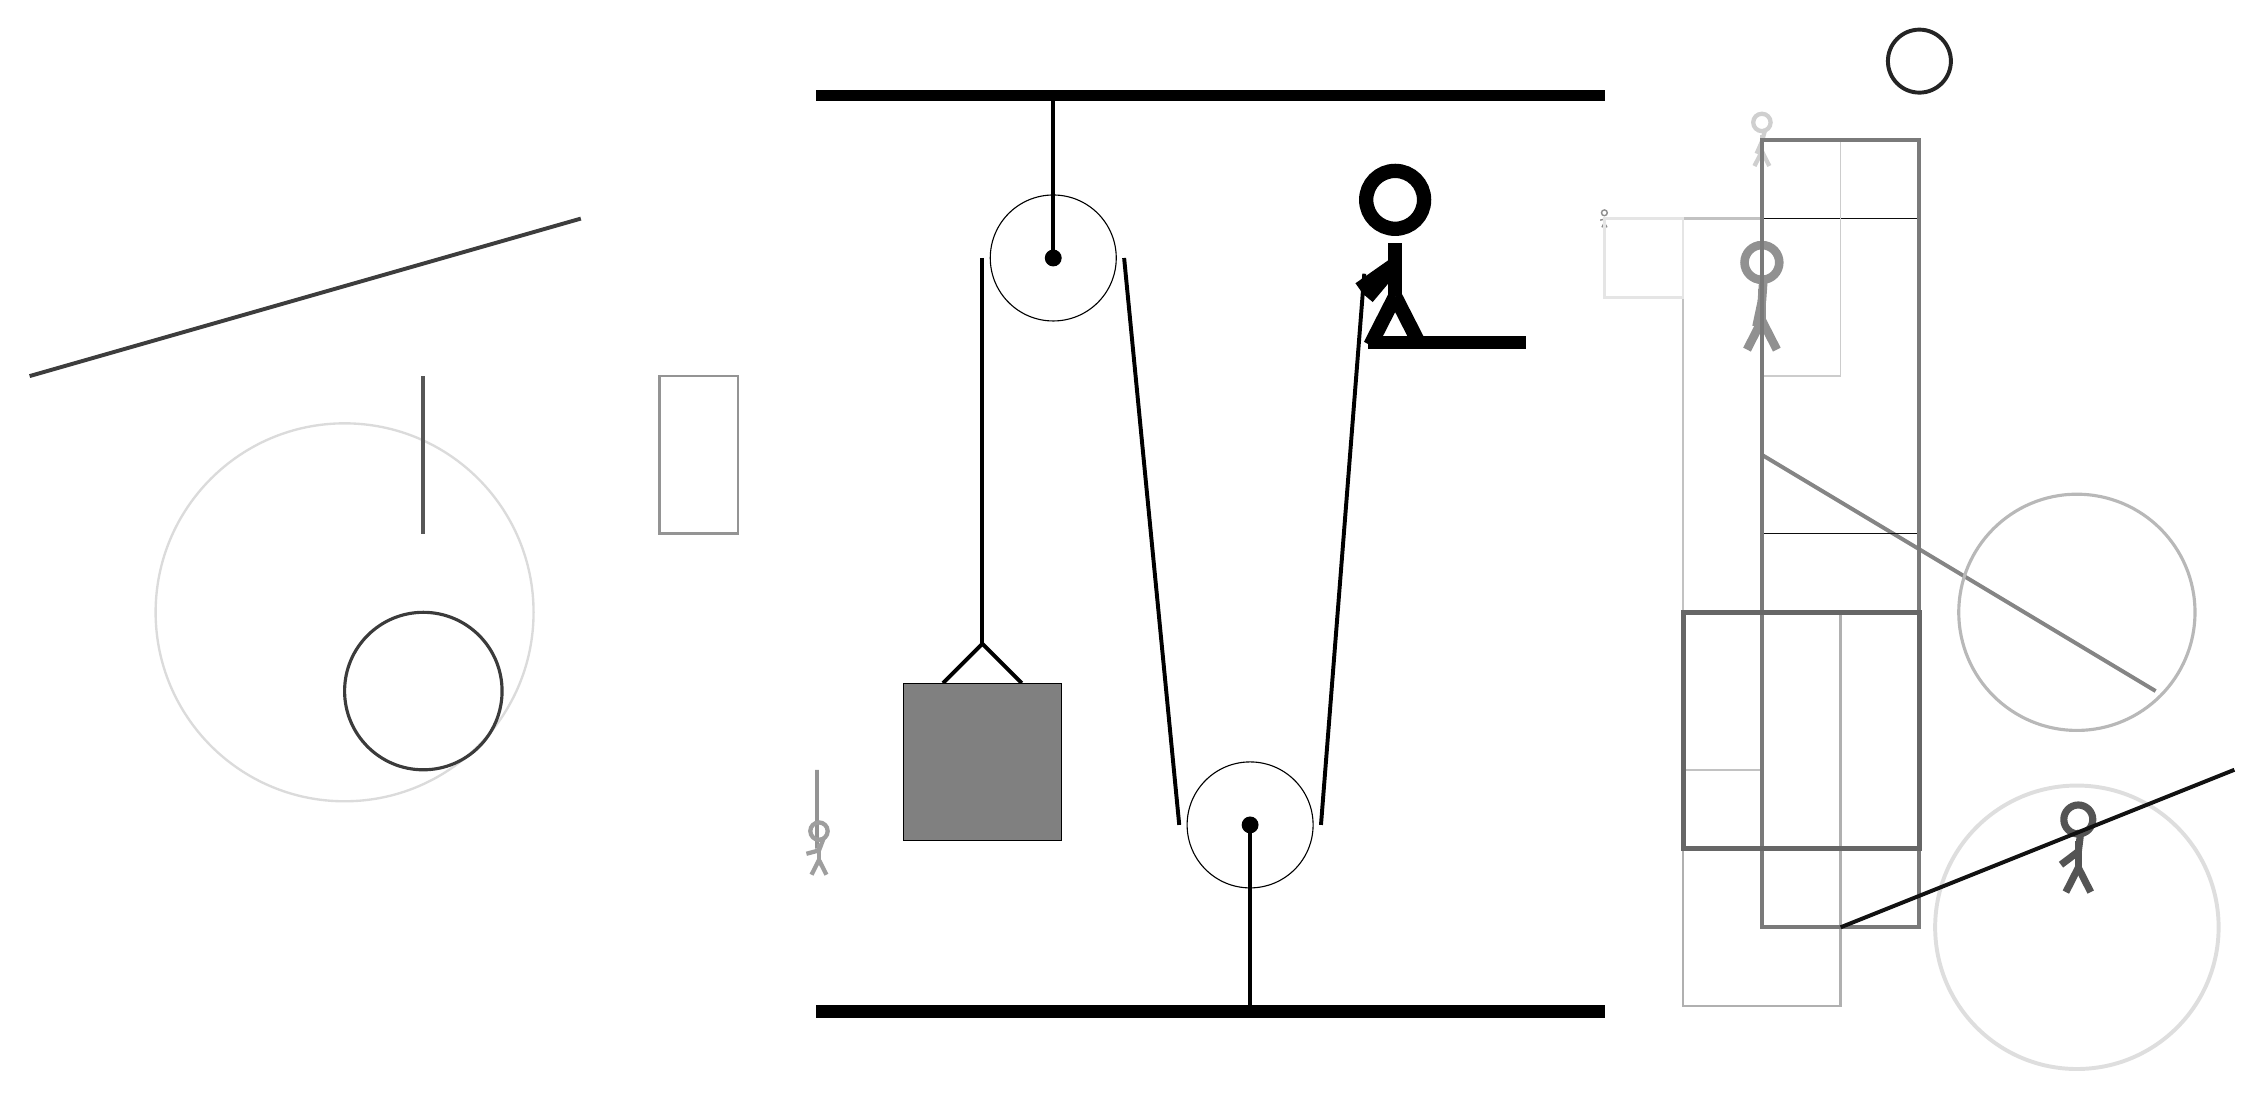
\begin{tikzpicture}
			%%%%% START %%%%%
			
			\draw[fill=black] (-2, 11.5) rectangle (8, 11.625);
			
			\draw (3.5, 2.3) circle (0.8);
			\draw[fill=black] (3.5, 2.3) circle (0.1);
			\draw[line width=0.5mm] (3.5, 2.3) -- (3.5, 0);
			
			\draw (1, 9.5) circle (0.8);
			\draw[fill=black] (1, 9.5) circle (0.1);
			\draw[line width=0.5mm] (1, 11.5) -- (1, 9.5);
			
			\draw[line width=0.5mm](-0.4, 4.1) --  (0.1, 4.6) -- (0.6, 4.1);
			\draw[fill=black!50] (-0.9, 4.1) rectangle (1.1, 2.1);
			
			\draw[line width=0.5mm](0.1, 9.5) -- (0.1, 4.6);
			\centerarc[line width=0.5mm](1, 9.5)(180:0:0.9)
			\draw[line width=0.5mm](1.9, 9.5) -- (2.6, 2.3);
			\centerarc[line width=0.5mm](3.5, 2.3)(180:360:0.9)
			\draw[line width=0.5mm](4.4, 2.3) -- (4.95, 9.3);
			
			\node at (5.3, 9.5) {\Strichmaxerl[10][35][-130]};
			\draw[fill=black] (5, 8.5) rectangle (7, 8.35);
			
			\draw[line width=0.5mm, color=black!42] (-2, 3) rectangle (-2, 2);
			
			\draw [line width=0.3mm, color=black!14](-8, 5) circle (2.4);
			\draw[line width=0.3mm, color=black!24] (10, 3) rectangle (9, 10);
			\draw[line width=0.5mm, color=black!48](10, 7) -- (15, 4);
			\draw[line width=0.5mm, color=black!63](-3, 7) -- (-3, 7);
			\draw[line width=0.3mm, color=black!42] (-3, 8) rectangle (-4, 6);
			\draw [line width=0.5mm, color=black!13](14, 1) circle (1.8);
			\node[line width=0.6mm, color=black!19] at (10, 11) {\Strichmaxerl[3][66][75]};
			\draw [line width=0.4mm, color=black!28](14, 5) circle (1.5);
			
			\draw[line width=0.3mm, color=black!31] (9, 0) rectangle (11, 5);
			\node[line width=0.7mm, color=black!43] at (10, 9) {\Strichmaxerl[6][78][86]};
			\draw[line width=0.2mm, color=black!95] (10, 10) rectangle (12, 6);
			\draw[line width=0.5mm, color=black!66](-7, 6) -- (-7, 8);
			
			\draw[line width=0.2mm, color=black!20] (10, 11) rectangle (11, 8);
			\draw [line width=0.4mm, color=black!75](-3, 0) circle (0.0);
			\draw[line width=0.5mm, color=black!52] (10, 11) rectangle (12, 1);
			
			\node[line width=0.4mm, color=black!44] at (8, 10) {\Strichmaxerl[1][12][1]};
			\node[line width=0.7mm, color=black!38] at (-2, 2) {\Strichmaxerl[3][15][69]};
			\draw [line width=0.4mm, color=black!77](-7, 4) circle (1.0);
			\draw[line width=0.3mm, color=black!10] (9, 9) rectangle (8, 10);
			\draw [line width=0.5mm, color=black!86](12, 12) circle (0.4);
			
			\draw[line width=0.5mm, color=black!76](-5, 10) -- (-12, 8);
			
			\node[line width=0.4mm, color=black!67] at (14, 2) {\Strichmaxerl[5][37][83]};
			\draw[line width=0.5mm, color=black!93](11, 1) -- (16, 3);
			\draw[line width=0.6mm, color=black!60] (9, 2) rectangle (12, 5);
			
			
			\draw[fill=black] (-2, 0) rectangle (8, -0.15);
			
			%%%%% END %%%%%
		\end{tikzpicture}
	\end{figure}	
\end{document}